\documentclass[10pt,aspectratio=169,serif]{beamer}

\usepackage[fontset=none, scheme=plain]{ctex}
\IfFontExistsTF{Songti SC}{%
	\setCJKmainfont{Songti SC}[AutoFakeSlant=0.2]%
	\setCJKsansfont{Songti SC}[AutoFakeSlant=0.2]%
}{%
	\setCJKmainfont{FandolSong-Regular}[Extension=.otf,BoldFont=FandolSong-Bold,AutoFakeSlant=0.2]%
	\setCJKsansfont{FandolSong-Regular}[Extension=.otf,BoldFont=FandolSong-Bold]%
}
\usepackage{amsmath,amssymb,graphicx,tikz,booktabs,multicol,calligra}
\usepackage{pgfplots}
\pgfplotsset{compat=1.18}
\usepackage{tcolorbox}
\tcbuselibrary{skins}
\usepackage{XyygU}
\usepackage{caption}
\captionsetup[figure]{name=图,labelsep=period}

\usetikzlibrary{arrows.meta,positioning,calc}

\setlength{\abovedisplayskip}{0pt plus 2pt minus 2pt}
\setlength{\belowdisplayskip}{0pt plus 2pt minus 2pt}

\title[幂函数练习]{3.3 幂函数（练习）}
\subtitle{幂函数的图象与性质}
\author{}
\institute{}
\date{2026-10-16}

\begin{document}

\begin{frame}
  \titlepage
\end{frame}

% ========== 第1题 ==========
\begin{frame}[t]{第1题：求幂函数解析式}
\textbf{1.} 已知幂函数 $y=f(x)$ 的图象过点 $(2,\sqrt{2})$，求这个函数的解析式。
\end{frame}

\begin{frame}[t]{第1题 解答}
\begin{tcolorbox}[colback=orange!10,colframe=orange,title=\textbf{解}]
设幂函数为 $f(x)=x^{\alpha}$。

\vspace{0.3em}
因其图象过点 $(2,\sqrt{2})$，代入得：
\[
2^{\alpha}=\sqrt{2}=2^{\frac12},
\]
所以 $\alpha=\dfrac12$。

\vspace{0.5em}
故所求函数解析式为
\[
\alert{f(x)=x^{\frac12}=\sqrt{x}},\quad x\ge 0.
\]
\end{tcolorbox}
\end{frame}

% ========== 第2题 ==========
\begin{frame}[t]{第2题：比较大小}
\textbf{2.} 利用幂函数的性质，比较下列各题中两个值的大小：

\vspace{0.5em}
(1) $(-1.5)^3$，$(-1.4)^3$；

\vspace{0.5em}
(2) $\dfrac{1}{-1.5}$，$\dfrac{1}{-1.4}$。
\end{frame}

\begin{frame}[t]{第2题 解答}
\begin{tcolorbox}[colback=orange!10,colframe=orange,title=\textbf{解}]
(1) 幂函数 $y=x^3$ 在 $\mathbf{R}$ 上单调递增。

\vspace{0.3em}
因为 $-1.5<-1.4$，所以 $(-1.5)^3\alert{<}(-1.4)^3$。

\vspace{0.8em}
(2) $\dfrac{1}{-1.5}=(-1.5)^{-1}$，$\dfrac{1}{-1.4}=(-1.4)^{-1}$。

\vspace{0.3em}
幂函数 $y=x^{-1}$ 在 $(-\infty,0)$ 上单调递减。

\vspace{0.3em}
因为 $-1.5<-1.4$，所以 $(-1.5)^{-1}\alert{>}(-1.4)^{-1}$，
即 $\dfrac{1}{-1.5}>\dfrac{1}{-1.4}$。
\end{tcolorbox}
\end{frame}

% ========== 第3题 ==========
\begin{frame}[t]{第3题：讨论 $f(x)=x^3$ 的性质}
\textbf{3.} 根据单调性和奇偶性的定义，讨论函数 $f(x)=x^3$ 的单调性，并判断其奇偶性。
\end{frame}

\begin{frame}[t]{第3题 解答}
\begin{tcolorbox}[colback=orange!10,colframe=orange,title=\textbf{解}]
\textbf{奇偶性：} 定义域为 $\mathbf{R}$，关于原点对称。
\[
f(-x)=(-x)^3=-x^3=-f(x),
\]
故 $f(x)=x^3$ 是 \alert{奇函数}。

\vspace{0.8em}
\textbf{单调性：} 任取 $x_1<x_2$，
\[
f(x_1)-f(x_2)=x_1^3-x_2^3=(x_1-x_2)(x_1^2+x_1x_2+x_2^2).
\]
因 $x_1-x_2<0$，而 $x_1^2+x_1x_2+x_2^2=\left(x_1+\dfrac{x_2}{2}\right)^2+\dfrac34x_2^2>0$（仅 $x_1=x_2=0$ 时取等），

\vspace{0.3em}
故 $f(x_1)-f(x_2)<0$，即 $f(x_1)<f(x_2)$，$f(x)=x^3$ 在 $\mathbf{R}$ 上 \alert{单调递增}。
\end{tcolorbox}
\end{frame}

\begin{frame}[t]{第3题 图象}
\begin{center}
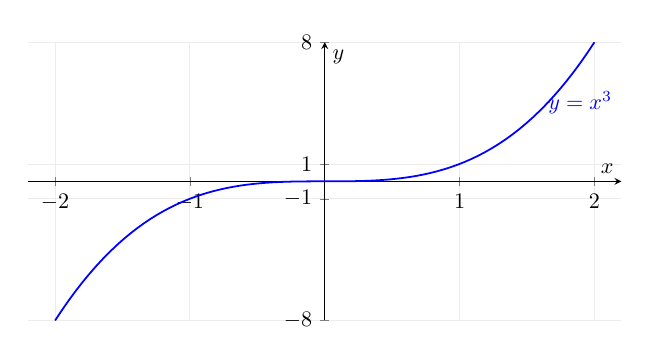
\begin{tikzpicture}[scale=0.8]
\begin{axis}[
    width=11cm, height=6cm,
    axis lines=middle,
    xlabel=$x$, ylabel=$y$,
    xmin=-2.2, xmax=2.2, ymin=-8, ymax=8,
    xtick={-2,-1,0,1,2},
    ytick={-8,-1,0,1,8},
    grid=major, grid style={gray!15},
]
\addplot[thick,blue,domain=-2:2,samples=80] {x^3};
\node[blue,right] at (axis cs:1.6,4.5) {$y=x^3$};
\end{axis}
\end{tikzpicture}
\end{center}
\end{frame}

\begin{frame}[c]
  \begin{center}
    {\Huge\calligra Thanks!}
  \end{center}
\end{frame}

\end{document}
